\documentclass[a4paper, 10pt]{article}

\usepackage[ansinew]{inputenc}			
\usepackage[german]{babel}		% for german	
\usepackage{graphicx}			
\usepackage{hyperref,breakurl}
\usepackage{amsmath}				
\usepackage{psfrag}

\addtolength{\textwidth}{2.1cm}
\addtolength{\topmargin}{-1.4cm}
\addtolength{\oddsidemargin}{-1.1 cm}
%\addtolength{\textheight}{2.5cm}

\pagestyle{plain} 					


\begin{document}

\date{22. Juli 2011}								
		

\title{
\textbf{Richtiges Zitieren zur\\ Sicherung guter wissenschaftlicher Praxis
\\[2ex]
{\small 
Lehrstuhl f\"ur Multimediakommunikation und
Signalverarbeitung\linebreak Universit\"at Erlangen-N\"urnberg\\
}}
}

\author{Rudolf Rabenstein}

\maketitle
\thispagestyle{empty} 			

\section{Einleitung}
\label{sec:intro} 

Die Universit\"at Erlangen-N\"urnberg hat Richtlinien zur Sicherung guter
wissenschaftlicher Praxis erlassen~\cite{FAU:wiss-Prax:2002}. Darin sind einige
Grunds\"atze des wissenschaftlichen Arbeitens und Publizierens niedergelegt,
aber auch das Verfahren bei Verdacht auf wissenschaftliches Fehlverhalten.

Einige dieser Grunds\"atze betreffen auch die Abfassung von Abschlussarbeiten
und der zugeh\"origen Ausarbeitungen. Daher behandelt der folgende Abschnitt
die Fairness bei wissenschaftlichen Publikationen, die sich in
korrekten Verweisen auf die Arbeiten anderer Autoren ausdr\"uckt. Eine
ausf\"uhrliche Literaturliste dient aber nicht nur der Fairness gegen\"uber
anderen Autoren.  Sie ist auch eine Dienstleistung f\"ur die Leser, denn nur so
k\"onnen sie die zitierten B\"ucher, Zeitschriftenartikel oder Web-Seiten 
selbst finden und lesen. Wissenschaftliche Arbeit erfordert die
\"Uberpr\"ufbarkeit der Ergebnisse und dazu geh\"ort der Zugang zu den Quellen
und
Vorarbeiten.

Um in der Ausarbeitung zu einem Seminarvortrag oder einer Bachelor- oder
Master-Arbeit die Publikationen anderer Autoren richtig zu zitieren, gen\"ugt
aber nicht nur der gute Wille zur Fairness gegen\"uber anderen Autoren. 
Die Erstellung, Pflege und richtige Nutzung einer
Literaturdatenbank erfordert einige Kenntnisse und ist nicht ganz einfach.
F\"ur Routineaufgaben gibt es dazu aber eine ganze Reihe von
Zusatzfunktionen von Textverarbeitungsprogrammen, Datenbankprogramme und
netz-basierte Suchm\"oglichkeiten. Einige wenige dieser Funktionen aus dem
\LaTeX-Kontext werden in einem weiteren Abschnitt besprochen. 

Dieser Text schlie{\ss}t selbstverst\"andlich mit einer umfangreichen Liste von
Literaturzitaten. Wie diese zustandekommen, kann man den Quelldateien zu diesem
Dokument entnehmen.


\section{Zitate von Ver\"offentlichungen anderer Autoren}

Zur Fairness bei wissenschaftlichen Publikationen enth\"alt \cite[\S4]{FAU:wiss-Prax:2002} Vorgaben 
\begin{itemize}
 \item 
zu Zitaten von Forschungsergebnissen und Ideen anderer Wissenschaftler und von
Publikationen anderer Autoren,
\item
zur Rolle von Mitautoren und deren Aufgaben und Verantwortung.
\end{itemize}
Speziell zu Ver\"offentlichungen anderer Autoren hei{\ss}t es dort, sie seien in "`geeigneter Weise zu zitieren''\cite[\S4(1)1]{FAU:wiss-Prax:2002}. Wie diese Vorgabe praktisch umzusetzen ist, wird hier beschrieben.

 \subsection{Fu{\ss}noten und Endnoten}

Welche Zitierweise in wissenschaftlichen Texten als geeignet gilt, unterscheidet
sich in den verschiedenen Disziplinen. In den Geisteswissenschaften sind
Fu{\ss}noten \"ublich, in denen nicht nur auf die Arbeiten anderer Autoren
verwiesen wird, sondern auch andere, zum laufenden Text geh\"orige Informationen
gegeben werden%
\footnote{Mitunter gilt eine Arbeit in den Geistes- und Rechtswissenschaften erst dann als "`wissenschaftlich", wenn sie m\"oglichst viele Fu{\ss}noten enth\"alt.}.

In technischen Texten sind dagegen Endnoten \"ublich, die am Ende des Dokuments erscheinen, oft in einem eigenen Abschnitt. Endnoten enthalten ausschlie{\ss}lich Quellenangaben der verwendeten Literatur. Auf erl\"auternde Fu{\ss}noten wird in technischen Dokumenten meist verzichtet, denn ein gut gegliederter Text braucht keine zus\"atzlichen Erkl\"arungen.

\subsection{Was wird zitiert?}

Grunds\"atzlich sind alle verwendeten Publikationen zu zitieren, unabh\"angig
davon, ob daraus ganze Textpassagen entnommen wurden oder ob auf darin
enthaltenen Ergebnisse oder Vorarbeiten verwiesen wird. Aber auch die Herkunft
von Formeln, Bildern,  Zeichnungen und Messwerten muss angegeben werden. Auf die
w\"ortliche Wiedergabe von l\"angeren Passagen aus fremden Texten sollte in
technischen Artikeln verzichtet werden. 

\subsubsection{Literatur aller Art}

Die f\"ur die eigene Arbeit verwendete Literatur muss so ausf\"uhrlich beschrieben werden, dass die Literaturangaben f\"ur eine Web- oder Bibliotheks-Recherche ausreichen. Dazu geh\"oren auf jeden Fall der Name des Autors oder der Autoren, der Titel der Ver\"offentlichung und das Erscheinungsjahr. Dazu kommen weitere Angaben, die vom Typ der Ver\"offentlichung abh\"angen (Buch, Zeitschriftenartikel, Konferenzband, Web-Seite, etc.). Beispiele sind in Abschnitt~\ref{sec:LaTeX} zu finden.

\subsubsection{Bilder und Zeichnungen}

Wenn Bilder, Zeichnungen und Grafiken aller Art eingescannt oder abfotografiert,
von Webseiten heruntergeladen, oder aus digitalen Dokumenten extrahiert wurden,
ist die Herkunft in der Bildunterschrift anzugeben, siehe Abb.~\ref{fig:2}. Dies
gilt auch, wenn Zeichnungen nach einer fremden Vorlage selbst angefertigt wurden
oder fremde Bilder und Zeichnungen durch eigene Zus\"atze erg\"anzt wurden.

\begin{figure}
\centerline{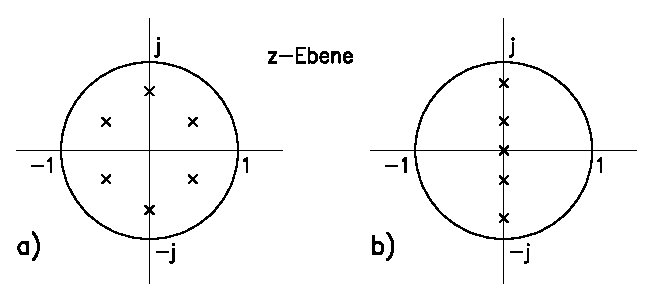
\includegraphics[width=0.5\textwidth]{fig/BILD3-49.eps}}
\caption{Polstellen von \"Ubertragungsfunktionen
rekursiver Halbbandfilter (aus~\cite{Schuessler:DSV2:2010}).}
\label{fig:2}
\end{figure} 

\subsubsection{Messwerte und andere Daten}

Auch f\"ur Messwerte, technische Angaben, Versuchsbedingungen etc., die aus anderen Publikationen entnommen sind, ist die Fundstelle so genau anzugeben, dass jeder Leser diese Angaben im Original \"uberpr\"ufen kann.

\subsubsection{Fachliches Allgemeinwissen}

Inhalte, die in vielen Lehrb\"uchern oder Grundlagenvorlesungen zu finden sind,
z\"ahlen zum fachlichen Allgemeinwissen und brauchen nicht zitiert zu werden.
Beispiele sind der Satz von Pythagoras, die Methode der kleinsten
Fehlerquadrate, das Abtasttheorem, oder das
Raleigh-Integral~\cite{Blauert:Acoustics:2009}. Trotzdem kann es sinnvoll sein,
ein allgemein zug\"angliches Lehrbuch als Quelle anzugeben. Dies ist dann ein
Service f\"ur die Leser, aber keine Erfordernis zur Fairness gegen\"uber
anderen Autoren.


\subsection{Wie wird zitiert?}
\label{ssec:wie}

F\"ur die Formulierung der Referenzen gibt es eine Vielzahl von Regeln, die aber oft von Verlag zu Verlag und von Zeitschrift zu Zeitschrift variieren. Dazu z\"ahlen
\begin{itemize}
 \item 
die Schreibweise der Autorennamen (Vornamen abgek\"urzt oder nicht, vor oder nach dem Nachnamen, mehrere Autoren durch \emph{und} oder durch Komma getrennt),
\item
der Schriftsatz des Publikationstitels (kursiv oder nicht),
\item
die Reihenfolge der weiteren Angaben (Jahreszahl, Seitenangaben, etc.)
\end{itemize}
und viele weitere Angaben. Dies mag kleinlich erscheinen, dennoch ist bei einer langen Literaturliste eine einheitliche Gestalt der Literaturangaben von gro{\ss}em Wert.

Ebenso ist es wichtig, dass die Nummerierung der Referenzen im Text mit der Literaturliste am Ende \"ubereinstimmt. Fehler an dieser Stelle k\"onnen gro{\ss}es Unheil anrichten, wie z.B. in~\cite[Kap.~15]{Coe:House_of_Sleep:1997} beschrieben.

Es ist nicht notwendig, sich mit diesen Regeln im Detail zu befassen, denn die
aktuellen Programme zur Textverarbeitung und zum Textsatz bieten automatische Formatierungshilfen. 
Ebenso gibt es die M\"oglichkeit, die einzelnen Bestandteile der Literaturangaben (Autor, Titel, etc.) in einer Datenbank zu verwalten. Einmal eingegeben, kann ein Datensatz so in mehreren Ver\"offentlichungen verwendet oder mit anderen Autoren ausgetauscht werden.
Diese M\"oglichkeiten werden im Weiteren anhand des Software-Pakets \LaTeX{}  erl\"autert.



\section{Wissenschaftliche Zitate mit \LaTeX}
\label{sec:LaTeX}

\LaTeX{} ist ein bekanntes Softwaresystem zum Text- und Formelsatz. Es ist
f\"ur verschiedene Plattformen frei verf\"ugbar und f\"ur technische und
naturwissenschaftliche Texte der de facto Standard. Viele Konferenzen und
Buchverlage erwarten die eingereichten Texte im \LaTeX-Format und stellen oft
auch eigene Vorlagen daf\"ur bereit. 

\LaTeX{} bietet verschiedene M\"oglichkeiten zur Eingabe einer Literaturliste.
Die weitreichendste und flexibelste dieser M\"oglichkeiten verwendet das
Zusatzpaket BibTeX und ist in den folgenden Abschnitten beschrieben.
Grundlegende Kenntnisse im Umgang mit \LaTeX{} werden dabei vorausgesetzt. 

\subsection{Literaturdatenbank}

\subsubsection{Bib-Dateien}

Die Arbeit mit BibTeX erfordert eine Literaturdatenbank, die aus einer oder
mehreren Dateien mit der Endung {\tt .bib} besteht. Eine Datei gen\"ugt;
mehrere Dateien erlauben die Aufteilung in verschiedene Themenbereiche.

Eine bib-Datei besteht aus Datens\"atzen unterschiedlichen Typs f\"ur
entsprechende Typen von Ver\"offentlichungen. Ein Eintrag f\"ur den Typ
\emph{Book} ist in Abb.~\ref{fig:3} gezeigt. Im laufenden Text wird dieser
Datensatz durch den Befehl \verb+\cite{Blauert:Acoustics:2009}+
angesprochen~\cite{Blauert:Acoustics:2009}. Die Referenzen am Ende dieses
Artikels wurden aus den Angaben in der Datei {\tt RichtigZitieren.bib} erzeugt.

\begin{figure}[hbt]
\begin{verbatim}
 @BOOK{Blauert:Acoustics:2009,
  title = {Acoustics for Engineers},
  publisher = {Springer},
  year = {2009},
  author = {Jens Blauert and Ning Xiang},
  address = {Berlin}
 }
\end{verbatim}
\caption{Eintrag in eine Literaturdatenbank im BibTeX-Format. Nach der Angabe
des Typs ({\tt BOOK}) folgt ein Schl\"ussel {\tt Blauert:Acoustics:2009} zur
Referenzierung. Daran schlie{\ss}en sich Felder mit den Angaben f\"ur Titel,
Verlag, Jahr, Autoren, etc. an.}
\label{fig:3}
\end{figure}


Eine bib-Datei (oder mehrere) dient als pers\"onliche oder
gemeinsam nutzbare Literaturdatenbank. Sie
kann f\"ur viele Texte verwendet werden. Dabei erscheinen im jeweiligen Text nur
die Eintr\"age, die dort durch einen Befehl
\verb+\cite{...}+ angesprochen werden. Mit bib-Dateien kann man auch bequem
Literaturangaben mit anderen Autoren austauschen.

Eine bib-Datei kann man mit jedem einfachen Text-Editor erzeugen und
bearbeiten. Dazu muss die Syntax der Datenbankeintr\"age beachtet werden. Die
f\"ur jeden Typ erforderlichen Pflichtfelder m\"ussen eingetragen werden,
weitere Angaben sind m\"oglich.


\subsubsection{Datenbank--Interface f\"ur BibTeX}

Einfacher ist der Umgang mit BibTeX-Dateien, wenn man ein Datenbank--Interface
verwendet, z.B. den sog. \emph{JabRef reference
manager}~\cite{sourceforge:jabref:2011}.
Aber auch hier sind die verschiedenen Typen von Ver\"offentlichungen zu
unterscheiden. Die wichtigsten sind:

\begin{description}
 \item[Article]
f\"ur Artikel in wissenschaftlichen Zeitschriften,
\item[Book]
f\"ur B\"ucher, die von einen Verlag in Verkehr gebracht werden.
\item[Inproceedings]
f\"ur Beitr\"age zu Konferenzen (sog. Konferenz-Paper),
\item[Electronic]
f\"ur Webseiten, die durch einen URL angesprochen werden.
 \end{description}

Beitr\"age zu Konferenzen (Typ \emph{Inproceedings}) erscheinen heute in
verschiedenen Formaten:
\begin{itemize}
 \item traditionell in einem gedruckten Tagungsband,
\item auf einem Datentr\"ager wie CD oder USB-Stick,
\item zum Herunterladen von der Konferenz-Webseite.
\end{itemize}
Die Organisation der digitalen Dokumente entspricht oft noch der herk\"ommlichen
gedruckten Version.
Wenn vorhanden, sollten daher auch bei rein digitalen Dokumenten noch
Seitenzahlen (z.B. des PDF-Dokuments) angegeben werden.

Bei Webseiten (Typ \emph{Electronic}) mit wechselnden Inhalten ist es
\"ublich,  Jahr und Monat des letzten Aufrufs mit anzugeben.

\subsubsection{Herkunft der Angaben f\"ur BibTeX-Datens\"atze}

Die Angaben f\"ur die BibTeX-Datens\"atze kann man auf verschiedene Weise
erhalten. Am einfachsten entnimmt man sie direkt aus dem vorliegenden Artikel
oder Buch. Viele Zeitschriften drucken diese Angaben in die Kopf- oder
Fu{\ss}zeile auf jeder Seite. Bei B\"uchern findet man die notwendigen Angaben
auf der Titelseite oder in den bibliographischen Angaben auf deren R\"uckseite.

Bequemer ist es, die fertigen Angaben aus entsprechenden Webseiten zu kopieren
oder zu laden. Dazu bieten viele akademische Institutionen auf ihren
Webseiten Ver\"offentlichungslisten mit fertigen BibTeX-Eintr\"agen an,
siehe z.B.~ \cite{LMS:Zeitschriften:2011}.
Ebenso kann man Zitate im BibTeX-Format aus digitalen Bibliotheken
herunterladen, siehe~\cite{IEEE:Xplore:2011}. Der Reference Manager JabRef 
leistet hier Hilfestellung mit enstprechenden Zusatzfunktionen.  


\subsection{Zitierstil}

Die Datenbankeintr\"age enthalten zwar die notwendigen Informationen f\"ur eine
ausf\"uhrliche Literaturliste, aber keine Angaben f\"ur  deren Formatierung (s.
Abschn.~\ref{ssec:wie}). Daf\"ur gibt es eigene Dateien ({\tt
.bst}) mit dem jeweiligen Bibliographiestil. Damit kann man eine
Literaturdatenbank f\"ur unterschiedliche Ver\"offentlichungen mit
unterschiedlichen Zitierstilen verwenden. Dieses Dokument benutzt den
Zitierstil f\"ur IEEE Transactions  in der Datei {\tt IEEEtran.bst}. Weitere
Dateien mit anderen Formatierungen erh\"alt man bei Buchverlagen und
Konferenzen. Es empfiehlt sich nicht, eigene bst-Dateien zu erstellen oder
vorhandene zu ver\"andern.

\subsection{Automatisches Erzeugen der Literaturliste}

Wenn eine Literaturdatenbank und eine Datei f\"ur den Zitierstil vorhanden
sind, werden diese am Ende des \LaTeX-Dokuments mit den Befehlen
\begin{verbatim}
\bibliographystyle{IEEEtran}
\bibliography{RichtigZitieren}
\end{verbatim}
eingebunden. Beim \"Ubersetzen des \LaTeX-Dokuments muss dann noch die
bib-Datei mit eingebunden werden. Dies geschieht in der verwendeten
Entwicklungsumgebung (z.B. Kile oder TeXnicCenter) oder auf der Kommandozeile
mit
\begin{verbatim}
latex RichtigZitieren
bibtex RichtigZitieren
latex RichtigZitieren
latex RichtigZitieren
\end{verbatim}
Die Endungen der Dateien \verb+RichtigZitieren.tex+ und
\verb+RichtigZitieren.bib+ werden weggelassen. Das Zusammenspiel der Programme
\verb+latex+ und \verb+bibtex+ verkn\"upft die \verb+\cite+-Befehle im Text mit
der automatisch angelegten Literaturliste an seinem Ende.

Nach dem Einf\"ugen oder Entfernen
von Referenzen (\verb+\cite+) muss nach \verb+bibtex+ der Befehl \verb+latex+
zweimal aufgerufen werden, damit die Nummerierung konsistent ist. Anderfalls
drohen Effekte wie in~\cite[Kap.~15]{Coe:House_of_Sleep:1997} beschrieben.


\subsection{Weitere Beispiele}

Hier sind noch einige weitere Beispiele f\"ur verschiedene Typen von
Ver\"offentlichungen aufgef\"uhrt. Sie sollen den Zusammenhang zwischen 
\begin{itemize}
 \item den Eintr\"agen in der Datei \verb+RichtigZitieren.bib+,
 \item dem in der Datei \verb+IEEEtran.bst+ definierten Zitierstil,
 \item den in der Datei \verb+RichtigZitieren.tex+ enthaltenen
\verb+\cite+-Befehlen und
\item dem Druckbild der Literaturliste
\end{itemize}
noch einmal verdeutlichen. Diese Dateien k\"onnen direkt auch als Vorlage f\"ur
die Ausarbeitung verwendet werden.


\begin{description}
\item[Article]

\begin{quote}
Ein Ansatz zur Videocodierung findet sich in~\cite{4703235}.
\end{quote}
Dieser BibTeX-Datenbankeintrag (vgl.~Abb.~\ref{fig:3}) stammt
von der Literaturdatenbank~\cite{IEEE:Xplore:2011}.
\begin{quote}
Ein Ansatz zur Videocodierung findet sich in~\cite{Li09laplacedistribution}.
\end{quote}
Dieser BibTeX-Datenbankeintrag stammt von der Literaturdatenbank~\cite{CiteSeer:2011}.
\item[Article]

\begin{quote}
Verfahren zur Unterdr\"uckung akustischer Echos mit nichlinearem Echopfad
auf der Basis von Volterra-Filtern erfordern einen hohen Rechenaufwand. Zu
dessen Reduktion wird in~\cite{5428855} ein Verfahren mit adaptiver Kombination
aus mehreren Volterra-Kernen vorgeschlagen.
\end{quote}

\item[Book]

\begin{quote}
F\"ur digitale Filter mit Tschebyscheff-Verhalten im Durchlass- und im
Sperrbereich (sog. Cauer-Filter oder elliptische Filter) gibt es geschlossene
Entwurfsverfahren~\cite{Schuessler:DSV2:2010}.
\end{quote}


\item[Inproceedings]

\begin{quote}
Die Genauigkeit von Verfahren zur Lokalisierung akustischer Quellen wird
m\"oglicherweise auch von Temperaturschwankungen beeinflusst, wie
in~\cite{5463320} behauptet wird.
\end{quote}

\item[Electronic]
\begin{quote}
Die Tagungsb\"ande der Konferenzen \emph{Digital Audio Effects} seit dem Jahr
1998 sind auf der Webseite~\cite{DAFX} frei zug\"anglich.
\end{quote}
\end{description}

Die aus diesen Angaben erzeugte Literaturliste enth\"alt allerdings noch einige Fehler, wie im
Folgenden zu sehen ist.

%%%%%%%%%%%%%%%%%%%%%%%%%%%%%%%%%%%%%%%%%%%%%%%%%%%%%%%%%%%%%%%%%%%%%%%%%%%%%%%%%%
% Die folgenden Befehle dienen nur zur Erläuterung fehlerhafter BibTeX-Datensätze.
% Für die Bearbeitung eines Seminarvortrags können sie gelöscht werden.
\renewcommand\refname{Literatur-Rohfassung}
\input{RichtigZitieren-roh.bbl}
\renewcommand\refname{Literatur}
%%%%%%%%%%%%%%%%%%%%%%%%%%%%%%%%%%%%%%%%%%%%%%%%%%%%%%%%%%%%%%%%%%%%%%%%%%%%%%%%%%


\section{Fehler in  der Literatur-Rohfassung}

Das Herunterladen von BibTeX-Datenbankeintr\"agen von Literaturdatenbanken
wie~\cite{IEEE:Xplore:2011} oder~\cite{CiteSeer:2011} ist zwar sehr bequem, f\"uhrt aber
nicht immer automatisch zu einer gut formatierten Literaturliste. Oft sind diese
Datenbankeintr\"age automatisch erzeugt und enthalten Unvollkommenheiten und Fehler.
Einige Beispiele sind in der obigen Rohfassung der Literaturliste zu sehen.

Die Referenzen~\cite{4703235} und~\cite{Li09laplacedistribution} zitieren dieselbe
Ver\"offentlichung, stammen aber aus verschiedenen Literaturdatenbanken. Keine der beiden ist
fehlerfrei:

\begin{description}\labelsep=4.5mm
 \item[\cite{4703235}]
  \begin{itemize}
  \item
  Der Name der Zeitschrift \emph{IEEE Transactions on Circuits and Systems for Video Technology} ist
  nicht in der \"ublichen Schreibweise angegeben. 
  \item 
  Der Name des Monats Februar ist klein geschrieben. Manche Style-Dateien korrigieren solche
  Eintr\"age, hier ist das aber nicht geschehen.
  \end{itemize}
 \item[\cite{Li09laplacedistribution}]
  \begin{itemize}
  \item 
  Namenszus\"atze (Student Member, Senior Member) sind f\"alschlicherweise als Namen weiterer
Autoren dargestellt  (S. Member).
  \item
  Die Angaben zum Band (vol.) und Nummer (no.) der Zeitschriftenausgabe fehlen, ebenso der Monat.
 \end{itemize}
 \end{description} 
\"Ahnliche Fehler finden sich in~\cite{5428855} und~\cite{5463320}.

Der Grund f\"ur diese Fehler kann an falschen BibTeX-Eintr\"agen oder an der Inkompatibilit\"at
von BibTeX-Eintrag und Style-Datei liegen. Jedenfalls m\"ussen die BibTeX-Eintr\"age von Hand
erg\"anzt und korrigiert werden. \"Uber die korrekte Schreibweise in jedem Einzelfall geben
einschl\"agige Anleitungen der Herausgeber von Zeitschriften oder Buchverlage Auskunft. Ein
Beispiel ist das IEEE Style Manual~\cite{IEEE_Style_Manual}.
%
F\"ur die Ausarbeitung gen\"ugt aber auch eine kritische Durchsicht und der
Vergleich mit den Literaturangaben am Ende dieses Artikels, evtl. mit Hilfe des Betreuers. Dazu ist
es notwendig, die Ausarbeitung so rechtzeitig vorzulegen, dass Korrekturen ohne Zeitdruck m\"oglich
sind.

Nach einer Korrektur der heruntergeladenen BibTeX-Eintr\"age erscheint die Literaturliste so wie
auf der letzten Seite. Die zur Veranschaulichung m\"oglicher Fehler doppelt eingetrage
Literaturstelle~\cite{4703235} und~\cite{Li09laplacedistribution} sieht nun genau gleich aus.
Solche Doppeleintr\"age sind daher nicht n\"otig, denn ein BibTeX-Eintrag kann
beliebig oft zitiert werden. Die Monatsnamen und die Abk\"urzung f\"ur \emph{Seiten} (pp.)
erscheinen in englischer Sprache weil eine Style-Datei f\"ur englisch-sprachige Zeitschriften
verwendet wurde.
%
Wie die BibTeX-Eintr\"age zur Literaturliste am Ende aussehen, ist der Datei
\verb+RichtigZitieren.bib+ 
zu entnehmen. Die ebenfalls vorhandene Datei
\verb+RichtigZitieren-roh.bib+ enth\"alt zum Vergleich noch die unbearbeiteten Datens\"atze der
Rohfassung.


\section{Zusammenfassung}

Die korrekte Angabe der Quellen in einer wissenschaftlichen Arbeit erfordert
die Sammlung und strukturierte Angabe von Literaturzitaten. Moderne Systeme zur
Textverarbeitung stellen dazu umfangreiche Hilfsmittel zur Anlage, Pflege
und Verwendung von Literaturdatenbanken bereit. Zusammen mit der Literatursuche
auf den einschl\"agigen Internetportalen und den vordefinierten
Formatierungshilfen von Buchverlagen und wissenschaftlichen Vereinigungen
stehen so m\"achtige Werkzeuge bereit, um den Anforderungen zur Sicherung der
guten wissenschaftlichen Praxis gerecht zu werden. Eine fehlerfrei und satztechnisch korrekte
Darstellung der Literaturliste erfordert aber oft noch eine manuelle Korrektur einzelner
Datens\"atze.


\bibliographystyle{IEEEtran}	% Zitierstil für IEEE Transactions
\bibliography{RichtigZitieren}	% BibTeX-Datei mit derLiteraturdatenbank



\end{document}
